\section{Aufbau}
\label{sec:Aufbau}

In Abbildung \ref{fig:schema} ist der Versuchsaufbau zur Beobachtung des Zeeman-Effekts einer Cadmium(Cd)-Lampe schematisch dargestellt.
Diese wird in das Magnetfeld eines Elektromagneten eingebracht und die entstehenden Emissionslinien transversal zum Magnetfeld durch eine Anordnung von Linsen kollimiert. Die parallelen Strahlen fallen auf ein Geradsichtprisma und werden so entsprechend ihrer Wellenlänge aufgespalten. Durch einen Polarisationsfilter und einen Einzelspalt werden die zu untersuchenden Spektrallinien extrahiert und mittels Linsen auf eine Lummer-Gehrcke-Platte abgebildet. Das entstehende Interferenzmuster wird mithilfe einer Digitalkamera aufgenommen.

\begin{figure}
\centering
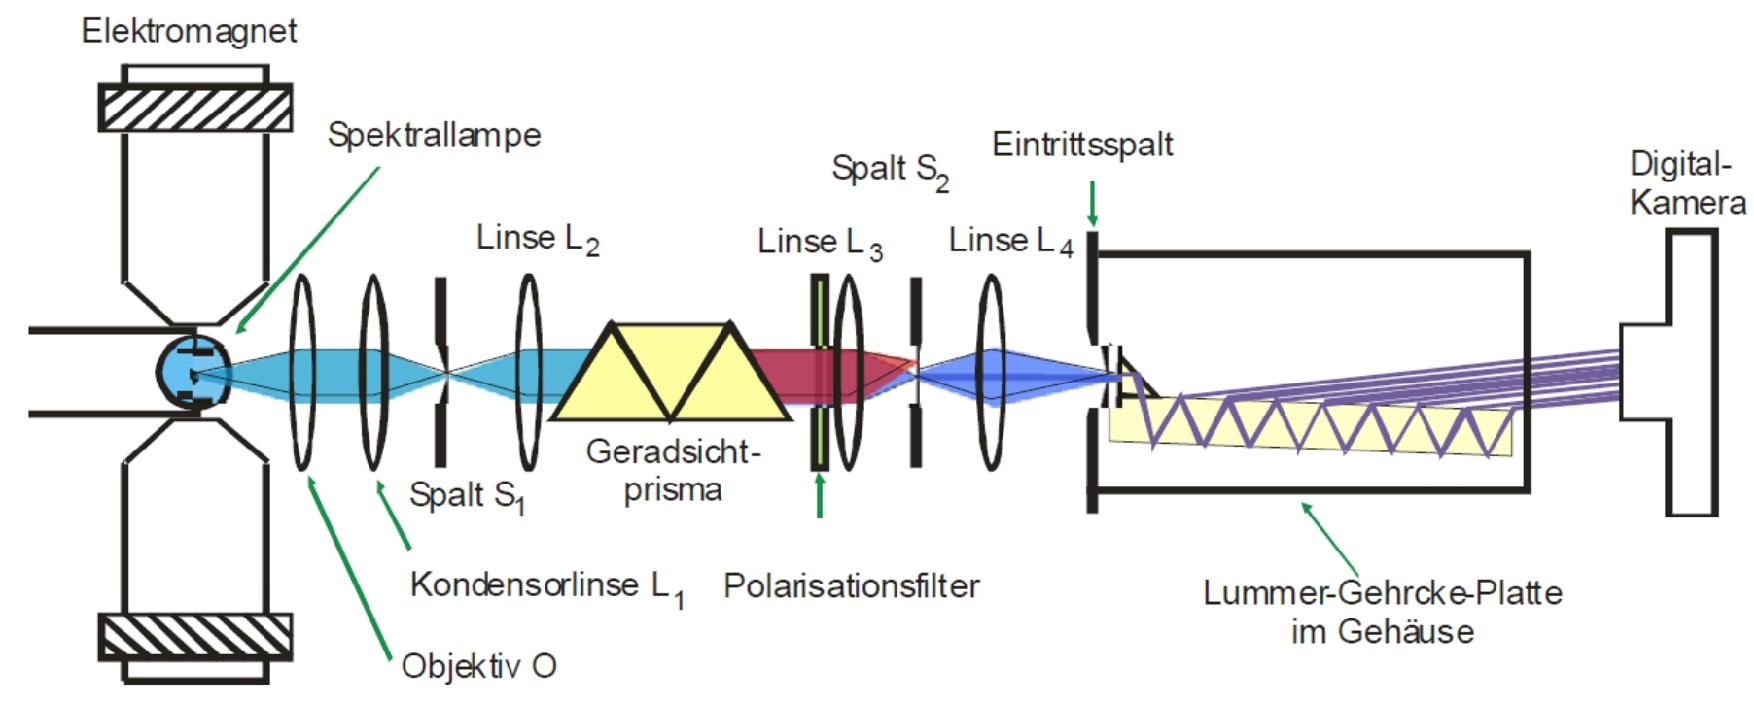
\includegraphics[width=0.8\textwidth]{build/schema.pdf}
\caption{Schematischer Aufbau zur Betrachtung des normalen und anormalen Zeeman-Effekts im Cadmium-Spektrum.\cite{V27}}
\label{fig:schema}
\end{figure}


%◘